\section{Models and representations}\label{sec:model}
Figure~\ref{fig:overview} summarizes the two retiming regimes and the implemented hybrid pipeline.
\subsection{Native events and temporal-grid packets}
The timestamp study uses native N-MNIST events $e_i=(x_i,y_i,p_i,t_i)$. Event identities, coordinates, polarity, labels and event count are immutable. Timestamps are assigned to ten equal-duration bins using the clean recording endpoints. The differentiable adapter has hard count accumulation in the forward pass and triangular interpolation weights for the backward pass. Counts are capped at 255 by the adapter. The hybrid frontend then applies $\min(X/8,1)$. These input transformations are model preprocessing; the preservation claim refers to the underlying events.

The grid study instead freezes a ten-bin equal-event-count representation. Each nonzero cell on a fixed spatial/polarity line is one amplitude-bearing packet. A binary packet has value one; an integer packet carries its complete cell count. A packet with count five remains a single packet carrying five during retiming. Collision-free capacity-one projection prevents packet splitting, merging, deletion, creation and amplitude changes. This distinction matters because multiple raw events can occupy one cell in the timestamp study, while one grid packet is indivisible in the second study.


\subsection{The implemented hybrid classifier}
The Conv/LIF extractor uses two $3\!\times\!3$ bias-free convolutions with 16 and 32 output channels, batch normalization and average pooling. LIF dynamics use decay 0.5. Time-averaged spike activations and the final membrane state are pooled to $4\!\times\!4$ spatial summaries and concatenated. A learned projection followed by tanh produces 32 latent features. A learned 32-to-8 projection and another tanh feed the circuit head. An additional learned 8-to-8 projection, initialized to the identity, produces bounded rotation angles.


For the latent vector $h\in\mathbb{R}^{32}$, the learned angle map is
\begin{equation}\label{eq:angles}
\begin{aligned}
 u&=\tanh(W_{32}h+b_{32}),\\
 a&=\pi\,\operatorname{clip}(W_8u+b_8,-1,1).
\end{aligned}
\end{equation}
The eight-qubit register starts in $|0\rangle^{\otimes 8}$. Each of two blocks applies an RY upload of each angle, an RZ upload scaled by a learned phase parameter, learned RY/RZ gates, and a ring of CNOT gates. Learned local RZ/RY rotations set the measurement basis. The model returns all 256 computational-basis probabilities to a linear ten-class classifier. All paths from the latent features to the logits pass through the circuit; there is no direct latent-to-logit branch.


\begin{equation}\label{eq:readout}
\begin{aligned}
p_k&=\left|\langle k|U_{\theta}(a)|0\rangle^{\otimes 8}\right|^2,
&& k=0,\ldots,255,\\
z&=W_{\mathrm{out}}p+b_{\mathrm{out}}.
\end{aligned}
\end{equation}
The backend is an analytic batched PyTorch state-vector simulation with complex64 amplitudes. Probabilities are computed exactly within numerical precision. The experiments do not involve quantum hardware, finite-shot readout or hardware noise. The name QSNN-v3 identifies this hybrid implementation and should not be interpreted as a network of physical quantum LIF neurons [R1].

\begin{table}[t]
\centering\caption{Trainable parameters of QSNN-v3.}\label{tab:parameters}
\small\begin{tabularx}{\linewidth}{L R}\toprule
\textbf{Component} & \textbf{Parameters}\\\midrule
Conv/LIF frontend and 32D summary & 37,792\\
Learned $32\to 8$ projection & 264\\
Angle map and quantum head & 136\\
Probability-to-logit classifier & 2,570\\\midrule
\textbf{Total} & \textbf{40,762}\\\bottomrule
\end{tabularx}
\vspace{3pt}\begin{minipage}{\linewidth}\footnotesize
The quantum head includes the learned $8\to8$ angle map, two upload blocks and learned measurement basis. Nontrainable BatchNorm buffers and state-vector storage are excluded [R1].
\end{minipage}\end{table}
\begin{figure*}[t]
\centering
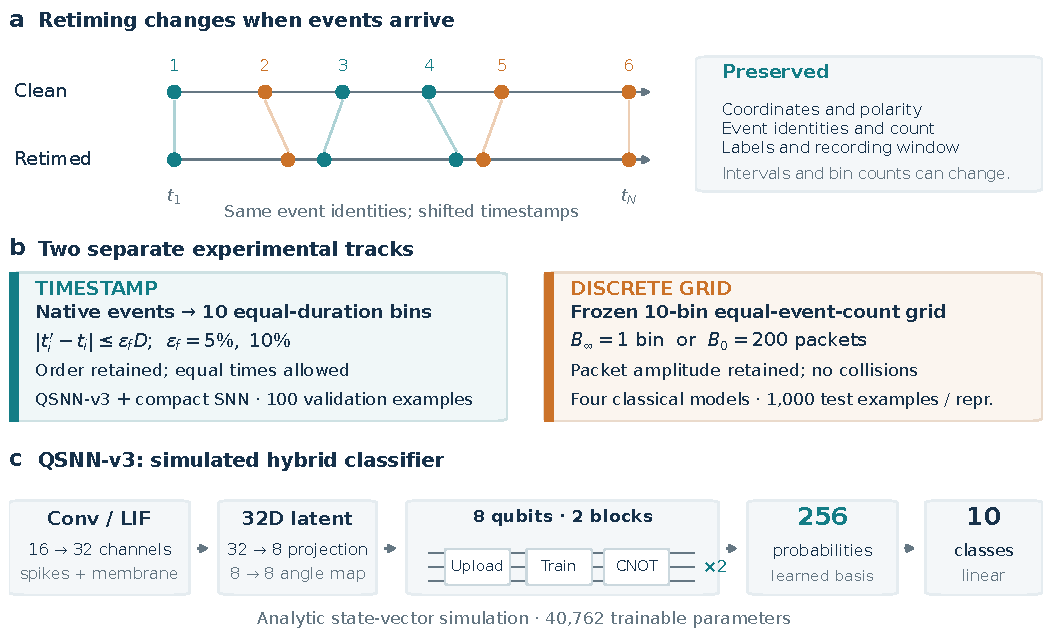
\includegraphics[width=\textwidth]{figures/fig01_overview.pdf}
\caption{Retiming protocols and implemented QSNN-v3. (a) Schematic retiming preserves event identity, coordinates, polarity, labels and count; intervals and bin counts can change. (b) The timestamp and discrete-grid studies use different representations, populations and budget units. Timestamp perturbations preserve nondecreasing order within the clean recording window; grid perturbations preserve indivisible packet amplitudes with collision-free scheduling. (c) Conv/LIF summaries pass through 32 latent features, learned 32-to-8 and 8-to-8 maps, and an eight-qubit, two-block circuit. The 256-probability readout alone feeds the ten-class classifier. The 40,762-parameter model uses analytic state-vector simulation. Circuit and event drawings are schematic. Sources: [R1--R4].}\label{fig:overview}
\end{figure*}

\subsection{State distance and classification margin}
\label{sec:margin_interpretation}
For the fixed trained model, let $\rho$ and $\rho'$ denote the clean and retimed quantum states before the fixed readout measurement, and let $q,q'\in\mathbb{R}^{256}$ be the corresponding outcome-probability vectors. Write the logits as $z(q)=Wq+b$, and define the clean pairwise margin against class $k\ne y$ by
\begin{equation}
m_{yk}(q)=(w_y-w_k)^\top q+b_y-b_k.
\end{equation}
Here $y$ is the clean predicted class, equal to the label on the attacked clean-correct subset, and $w_k$ is row $k$ of $W$. Measurement cannot increase trace distance, hence
\begin{equation}
\tfrac12\|q-q'\|_1\leq D_{\mathrm{tr}}(\rho,\rho'),
\qquad
D_{\mathrm{tr}}(\rho,\rho')=\tfrac12\|\rho-\rho'\|_1.
\end{equation}
The state norm is the trace norm; for probability vectors it is the ordinary $\ell_1$ norm. Combining this inequality with H\"older's inequality gives
\begin{equation}
\begin{split}
m_{yk}(q')\geq m_{yk}(q)\\
{}-2\|w_y-w_k\|_\infty D_{\mathrm{tr}}(\rho,\rho').
\end{split}
\label{eq:state_margin}
\end{equation}
Thus a sufficient condition for retaining class $y$ is that the right-hand side remain strictly positive for every $k\ne y$. To see this, subtract the two affine margins and bound the resulting inner product by $\|w_y-w_k\|_\infty\|q'-q\|_1$; positivity of all pairwise margins then preserves the argmax.

This observation separates state displacement from decision failure. A larger state distance need not cause a label change, and a small clean margin can make a smaller displacement consequential. Equation~\eqref{eq:state_margin} is a conditional interpretation of the implemented readout, not a certified timestamp radius: no uniform bound from admissible event retiming through the classical frontend to $D_{\mathrm{tr}}$ has been established here. The final-model campaign also does not report the per-example states needed to evaluate this condition. Its connection to quantum robustness theory is therefore conceptual rather than an application of an existing certificate \cite{dowling2026guarantees}.
